\documentclass{ximera}


\begin{document}
\input plot


%\begin{figure}
  %  \begin{gnuplot}[terminal=latex]
   %     plot [0:2*pi] x**2, cos(x)
    %\end{gnuplot}
%\end{figure}

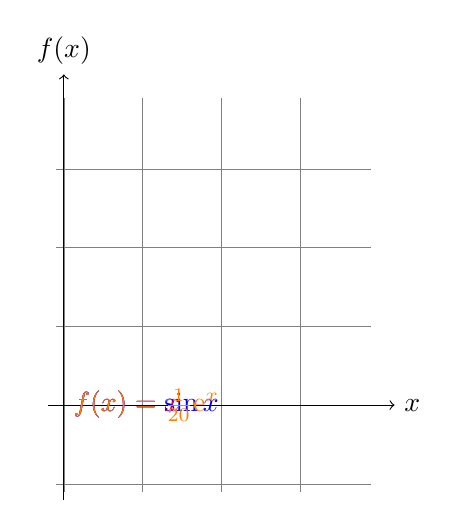
\begin{tikzpicture}[domain=0:4]
    \draw[very thin,color=gray] (-0.1,-1.1) grid (3.9,3.9);
    \draw[->] (-0.2,0) -- (4.2,0) node[right] {$x$};
    \draw[->] (0,-1.2) -- (0,4.2) node[above] {$f(x)$};
    \draw[color=red] plot[id=x] function{x} 
        node[right] {$f(x) =x$};
    \draw[color=blue] plot[id=sin] function{sin(x)} 
        node[right] {$f(x) = \sin x$};
    \draw[color=orange] plot[id=exp] function{0.05*exp(x)} 
        node[right] {$f(x) = \frac{1}{20} \mathrm e^x$};
\end{tikzpicture}

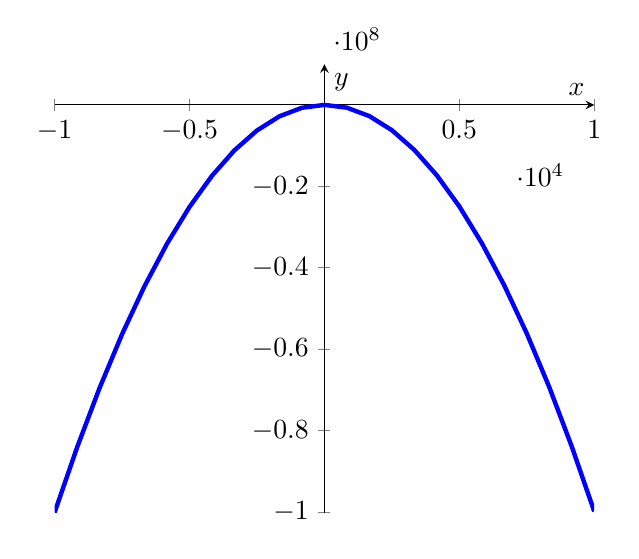
\begin{tikzpicture}
\begin{axis}[
        axis x line=middle, 
        axis y line=middle, 
        ymax=0.1E8, ylabel=$y$, 
        xlabel=$x$
        ]
    \addplot[domain=-10000:10000, blue, ultra thick] {14*x - x^2};
\end{axis}
\end{tikzpicture}

\end{document}
